\chapter{Systemarchitektur}
\label{chapter:systemarchitekur}

In den Kapiteln zuvor wurde in das Thema durch Grundlagen und eine Vorstellung der einzelnen Streaming Frameworks eingeführt. Dieses Kapitel beschreibt eine Methode zur Messung der Performance. Es wird zunächst das Messverfahren gezeigt, die Messumgebung und die Anforderungen an die Prototypen beschrieben. Um einem Vergleich zwischen den Streaming Frameworks auf Entwicklungsebene näher zu kommen, ist es notwendig eine allgemeine Anwendung in einer homogenen Umgebung zu entwickeln und bereitzustellen. Dazu werden zuerst die funktionalen Anforderungen und anschließend die nichtfunktionalen Anforderungen in schriftlicher und darstellerischer Form beschrieben.

\section{Funktionale Anforderung}
\label{sec:funktAnforderung}
Die funktionalen Anforderungen tragen dazu bei die Anwendung zu implementieren. In den folgenden Listen werden Kriterien für die Prototypen der einzelnen Streaming Frameworks definiert. Das Use-Case-Diagramm zeigt die Muss-Kriterien für den Anwender in Abbildung \ref{fig:useCaseMussKriterien}

\textbf{Muss-Kriterien:}
\begin{description}
  \item[M1] Paketierung der Implementierungen mit Apache Maven	
	\item[M2] Ausführung der Implementierungen unter Java und dem Betriebssystem Linux
	\item[M3] Ausführung einer Implementierung auf einem Single-Node-Cluster	
	\item[M4] Ausführung einer Implementierung von konstanter Größe von 100 Byte-Daten (statischer Payload)
	\item[M5] Ausführung einer Implementierung von variabler Größe von Daten (dynamischer Payload)
	\item[M6] Aufnahme von Daten: aktueller Nachrichten pro Sekunde und CPU-Belastung während der Ausführung einer Implementierung in  separaten Dateien 
	\item[M7] Während der Ausführung, anzeige der Daten pro Streaming Framework auf einer Webseite - Übersichtsseite
\end{description}

\textbf{Soll-Kriterien:}
\begin{description}
  \item[S1] Ausführung einer Implementierung auf verschiedenen Rechnersystemen (Professional Workstation, Notebook, Virtuelle Maschine)
	\item[S2] die Dynamische Implementierungen sollen Wörter aus einem offen und frei zugänglichen großen Datensatzes zählen und die Anzahl der höchsten 5 Wörter, sowie das Wort selbst pro Sekunde automatisch anzeigen
	\item[S3] Die Inhalte auf der Webseite sollen über Javascript-Trigger aktualisiert werden
\end{description}

\textbf{Kann-Kriterien:}
\begin{description}
  \item[K1] Ausführung der Implementierungen auf Multi-Node-Cluster
	\item[K2] Ausführung auf proprietären Betriebssystemen
\end{description}

\textbf{Abgrenzungskriterien:}
\begin{description}
  \item[A1] Für die prototypische Entwicklung werden erst in einem weiterführenden Konzept Unit- und Verhaltens-Tests eingesetzt
	\item[A2] Die Darstellung von Information auf einer Webseite benötigt beim Prototypen keine Serverseitige Absicherung
\end{description}


\begin{figure}[htb!]
\centering
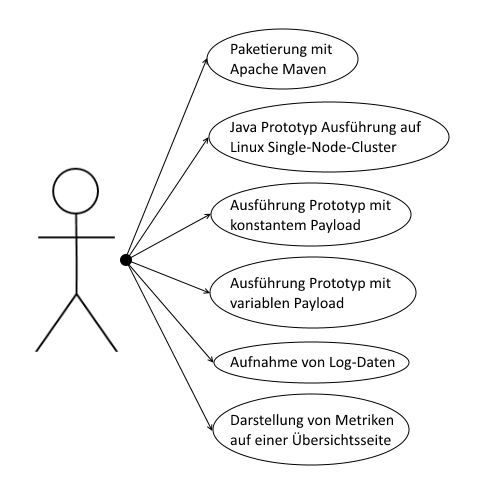
\includegraphics[width=0.65\textwidth]{bilder/useCaseMussKriterien.png}
\caption{Muss-Kriterien Use-Case-Diagramm
\label{fig:useCaseMussKriterien}}
\end{figure}

Nachdem die Kriterien vorgestellt wurden wird als nächste der Einsatzbereich und die Umgebung gezeigt.

\section{Nichtfunktionale Kriterien}
\label{sec:nichtFunktAnforderung}

Die Implementierungen der Prototypen werden hauptsächlich in einem wissenschaftlichen Studium eingesetzt. Als Zielgruppe können Wissenschaftler in der Informationstechnologie, Datenanalysten und Entwickler aus dem Bereich der Datenverarbeitung von zeitkritischen Daten und der Daten einer großen Menge, ein Interesse finden. Betrieben werden die Prototypen auf einem Notebook, in einer virtuellen Instanz und auf einer professionellen Workstation. Alle Rechnereinheiten werden über ein Switch verkabelt. Dabei wird ein homogenes Netz gebildet. 

Um Störgrößen zu vermeiden ist eine Verbindung in das Internet und das Intranet nicht vorgesehen und eine feste Verdrahtung essentiell. Kabellose Verbindungen werden aufgrund größerer Störempfindlichkeit wie zum Beispiel Kanalauslöschung nicht unterstützt. Das System wird mit kostenloser Open-Source Software entwickelt, dabei wird auf eine gute Wartbarkeit und Performance geachtet.

Angeschlossene Fremdrechner benötigen für die Darstellung der Übersichtsseite einen aktuellen Webbrowser\footnote{Webbrowser: \url{https://www.mozilla.org/de/firefox/desktop/}}. Die Nachrichten werden innerhalb der Streaming Frameworks binär und nach außen, zur Übersichtsseite als \gls{glo:json} übertragen. Für die Eingabedaten wird ein freies, offenes und großes Shakespeare-Datensatz \citeint{dataset:shakespeare:1994:CWW} benutzt. Bevor die Prototypen dokumentiert werden, wird der mögliche Probleme und Lösungsansätze vorgestellt.

\section{Probleme und Lösungsansätze}
\label{sec:loesungsansatz}

Für die Entwicklung geeigneter Prototypen sind bezogen auf die Anforderungen mögliche Konflikte vor der Implementierung zu lösen. Das Kapitel \ref{chapter:vorstellung} hat die Streaming Frameworks vorgestellt und konnte unterschiedliche Implementierungssprachen zeigen. So werden von den Streaming Frameworks unterschiedliche Programmierschnittstellen bereitgestellt. Aufgrund der prototypischen Entwicklung steigt die Komplexität und Übersicht, die Implementierungen für die Streaming Frameworks in ein Anwendungsprojekt zu packen. Da alle Streaming Frameworks die Java Plattform unterstützen, wird für die Entwicklung der Prototypen in einzelnen Java-Projekten entschieden. Durch Trennung der Verarbeitungslogik und der Ein- und Ausgabeformatierung in den Prototypen können Erweiterungen an gezielten Stellen im Quelltext effizient erfolgen. Da die Implementierungen nacheinander erfolgen, können so gewonnene Erkenntnisse in die bestehenden Implementierungen einfach übernommen werden. 

Durch die unterschiedlichen Streaming Frameworks werden ebenfalls unterschiedliche Bereitstellungsmechanismen eingesetzt. In Apache Storm wird zum Beispiel über ein Kommando in der Shell die Anwendung im Cluster bereitgestellt. Apache Flume zum Anderen benötigt zuerst eine Konfiguration, die anschließend über die Shell gestartet wird. Um die Komplexität weiterhin in der Entwicklung und Bereitstellung der Prototypen klein zu halten, ist ein gemeinsames Konzept für die Java-Paketierung ein wichtiges Instrument. Mit Hilfe von Apache Maven kann durch die Deklaration der Bereitstellung in einer Konfigurationsdatei\footnote{Die Konfigurationsdatei von Apache Maven heißt pom.xml und liegt in der ersten Ebene des Projektarchivs. Die Datenstruktur der Konfiguration besteht aus \gls{glo:xml}-Auszeichnungen. }, die Erstellung der einzelnen Prototypen von der Entwicklung getrennt und einheitlich erzeugt werden.

Mit den unterschiedlichen Streaming Frameworks werden teilweise unterschiedliche Logging-Frameworks eingesetzt. Damit bei der Abnahme des IST-Zustands und bei der Laufzeitdiagnose ein einheitliches Konzept verwendet wird, die Einarbeitungszeit in das Logging-Framework klein bleibt und um das Logging effizient zu halten, soll das Logging Framework Apache Log4j\footnote{Apache Log4j: \url{http://logging.apache.org/log4j/2.x/}} eingesetzt werden. Dabei soll die Weitergabe der Logging-Daten an die Übersichtsseite über das WebSocket-Protokoll erfolgen. Durch den Einsatz von WebSocket und Javascript EventHandler ist ein \textit{PageRefresh}\footnote{Ein \textit{PageRefresh} entspricht einem Neuladen der Webseite.} der Übersichtsseite nicht nötig. Die IST-Werte werden somit, sobald Werte eintreffen, auf der Übersicht durch Javascript Trigger aktualisiert.

Eine zeitgleiche Ausführung aller Streaming Frameworks auf einer Maschine kann zu unvorhergesehenen Ergebnissen bzw. Problemen führen. Auch für den Vergleich muss die Voraussetzung für die Messung gleich sein. Um die Messung möglichst gleich und Störeinflüsse gering zu halten, sollen alle Prototypen nacheinander auf je einer Maschine ausgeführt werden.

Für die \gls{glo:sdms} wurde der \gls{glo:lrb} von Arasu et al. \citelit[S. 488, Kap. 3.3]{linearRaod} entwickelt, um einen großen Umfang von Datenströmen und historische Daten zu verarbeiten. Das Ziel beim \gls{glo:lrb} ist die Ermittlung des \textit{L}-Rating eines \gls{glo:sdms}. In vier Schritten wird der \gls{glo:lrb} ausgeführt. Zuerst werden mit dem \textit{Historical data generator} historische Daten in einer Datei erzeugt. Anschließend werden mit dem \textit{Traffic simulator} und dem Data driver die \textit{L}-Daten in eine Datei geschrieben. Mit dem Start des \gls{glo:lrb} werden Ausgabedaten mit Zeitstempel geschrieben. Abschließend werden mit dem \textit{Validationtool} die Antwortzeiten und die Genauigkeit der Ausgabedaten geprüft und das \textit{L}-Rating bestimmt. 

Da die Implementierung des \gls{glo:lrb} in der Programmiersprache \gls{glo:coo} besteht, muss eine umfangreiche Portierung des Quelltextes in Java erfolgen. Für die Überführung des Quelltextes sind geeignete Qualitätssicherungen notwendig. An dieser Stelle wird nur ein Teilaspekt des \gls{glo:lrb} in Java entwickelt. Für den Benchmark in Java wird in den Prototypen einmal eine Methode für das Verarbeiten von konstanten 100 Byte Daten 240 Sekunden lang implementiert und in der zweiten Methode werden Wörter aus Texten mit variable Wortlänge gezählt und die Top-K-Werte pro Sekunde 240 Sekunden lang bestimmt. 

In diesem Kapitel wurden mögliche Probleme beim Betrieb oder während der Entwicklung erläutert und es wurden Lösungsansätzee vorgestellt. Im nächsten Kapitel wird der Systementwurf für die Prototypen gezeigt.

\section{Systementwurf}
\label{sec:systementwurf}

Im Bezug auf den die Anforderungen aus Kapitel \ref{sec:funktAnforderung} und \ref{sec:nichtFunktAnforderung} wird in diesem Kapitel ein Überblick über den Systementwurf gegeben. Dabei werden weiterführende Details der einzelnen Prototypen im Kapitel \ref{chapter:prototypeDocumentation} vorgestellt. Zuerst werden die eingesetzten Komponenten in einem Schaubild dargestellt und die Zusammenhänge erläutert.  

\begin{figure}[htb!]
\centering
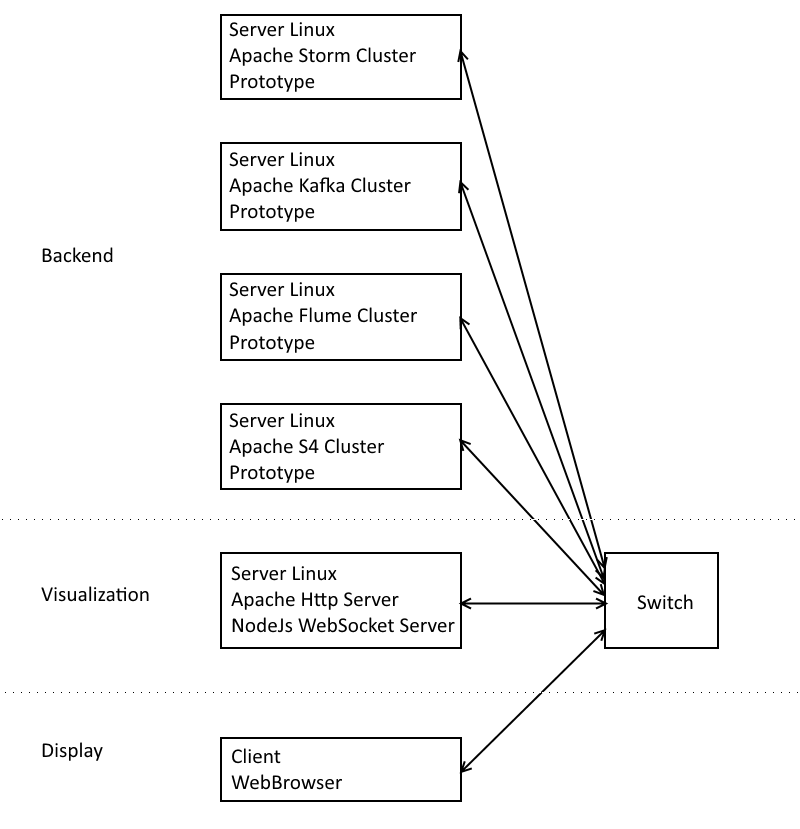
\includegraphics[width=0.75\textwidth]{bilder/Systementwurf.png}
\caption{Systementwurf
\label{fig:systementwurf}}
\end{figure}

In Abbildung \ref{fig:systementwurf} werden in drei Schichten verschiedene Arbeitsbereiche eingeteilt. Die obere Schicht wird als \textit{Backend} bezeichnet. Im \textit{Backend} werden die Cluster der einzelnen Streaming Frameworks in separaten Server-Maschinen betrieben. Auch die Prototypen der Streaming Frameworks werden im \textit{Backend} bereitgestellt. Die mittlere Schicht stellt die Anwendungschicht dar und wird als Visualization bezeichnet. In der \textit{Visualization} wird ein Apache Http Web Server\footnote{Apache Httpd Web Server: \url{http://httpd.apache.org/}} für die Bereitstellung der Webseite zur Übersicht und ein NodeJs\footnote{NodeJs ist eine Javascript Platform für die Entwicklung schneller und skalierter Netzwerkanwendungen. \url{http://nodejs.org/}} WebSocket\footnote{NodeJs WebSocket module für die Client-Server Entwicklung: https://www.npmjs.org/package/nodejs-websocket/} Server für die Verteilung der Log-Daten eingesetzt. Die untere Schicht stellt den Anwender dar und wird als \textit{Display} bezeichne. Im \textit{Display} wird ein Webbrowser aufgerufen um die \textit{Visualization} aus der mittleren Schicht anzuzeigen. Alle drei Schichten werden über \gls{glo:tcp}/\gls{glo:ip} durch den \textit{Switch} verbunden. Damit die Maschinen untereinander Daten austauschen können, wird jeder Maschine eine eindeutige \gls{glo:ip}-Adresse zugeordnet. Das folgende Kapitel \ref{sec:systemspezifiaktion} stellt anhand des Systementwurfs die Systemspezifikation vor.


\section{Systemspezifikation}
\label{sec:systemspezifiaktion}

Für die Ausführung der Prototypen in einem Single-Node-Cluster kommen Zwei Systeme zum Einsatz. Ein High End-Workstation und ein Low End-Workstation. Für das High End-Workstation wird eine starke \gls{glo:cpu} und hohe Anzahl von \gls{glo:ram}. In Tabelle \ref{tab:hiendwork} werden die Maschineneigenschaften der High End Maschine aufgestellt. Beim Low End-Workstation dagegen kommt eine schwace \gls{glo:cpu} mit einer kleinen Anzahl an \gls{glo:ram} zum Einsatz. Die Tabelle \ref{tab:loendwork} zeigt die Werte der der Low End Maschine. Beide Maschinen sind mit einem Switch über die Netzwerkkarten\footnote{Die Netzwerkkarten haben eine Bandbreite von 1 GBit/s} miteinander verbunden. 

\begin{table}[ht]
	\centering
		\begin{tabular}{@{}ll@{}} \toprule
			\textbf{Maschineneigenschaft} &  \\ \midrule
			\gls{glo:cpu} Bezeichnung & AMD FX-8350 \\
			\gls{glo:cpu} Taktfrequenz & 4 GHz \\
			\gls{glo:cpu} Anzahl Kerne & 8 \\
			CPU Einführung & Quartal 4 in 2012 \\
			\gls{glo:ram} & 16 GByte \\
			Netzwerkkarte & 1 GBit \\
			\bottomrule			
		\end{tabular}
	\caption{High End Workstation Eigenschaften}
	\label{tab:hiendwork}
\end{table}

\begin{table}[ht]
	\centering
		\begin{tabular}{@{}ll@{}} \toprule
			\textbf{Maschineneigenschaft} &  \\ \midrule
			\gls{glo:cpu} Bezeichnung & Intel i5-480M \\
			\gls{glo:cpu} Taktfrequenz & 2,66 GHz \\
			\gls{glo:cpu} Anzahl Kerne & 2 \\
			CPU Einführung & Quartal 1 in 2011 \\
			\gls{glo:ram} & 4 GByte \\
			Netzwerkkarte & 1 GBit \\
			\bottomrule			
		\end{tabular}
	\caption{Low End Workstation Eigenschaften}
	\label{tab:loendwork}
\end{table}

Die Maschinen werden mit einer Festplatte über \gls{glo:esata}\footnote{\gls{glo:esata} Spezifikation: \url{https://www.sata-io.org/esata}} angeschlossen. Für den Vergleich wird nur eine Festplatte mit dem eingesetzten Betriebssystem und den Prototypen betrieben. Mit \gls{glo:esata} ist es einfach die Maschinen durch Wechseln des Anschlusses zu tauschen. Die Tabelle \ref{tab:festplatte} zeigt die Geräteeigenschaften der Festplatte. In Anhang \ref{section:zusSystemarchitektur} Abbildung \ref{fig:festplatteLeistungstest} wird ein Leistungstest der Festplatte aus Tabelle \ref{tab:festplatte} angehängt. Darin wird das Ergebnis eines Lese- und Schreib-Vergleichstest gezeigt. Die Mittelwerte aus dem Leistungstest wurden aus dem Ausschnitt Abbildung \ref{fig:festplatteLeistungstest} in die Tabelle \ref{tab:festplatte} übernommen.

\begin{table}[ht]
	\centering
		\begin{tabular}{@{}ll@{}} \toprule
			\textbf{Geräteeigenschaft} &  \\ \midrule
			Festplattenbezeichnung & Hitachi HDS721616PLA380 \\
			Anschlusstyp & \gls{glo:esata} \\
			Größe & 165 GByte \\
			Spindelgeschwindigkeit & 7200 rpm \\
			Mittlere Lesegeschwindigkeit & 62,1 MByte/s \\
			Mittlere Schreibgeschwindigkeit & 52,1 MByte/s \\
			Mittlere Zugriffszeit & 13,6 s \\
			\bottomrule			
		\end{tabular}
	\caption{Eigenschaften Festplatte}
	\label{tab:festplatte}
\end{table}

Als Betriebssystem wird die Linux\footnote{Linux Kernel \url{https://www.kernel.org/}} Distribution Debian\footnote{Linux Distribution Debian: \url{http://www.debian.org/}} in der Version 7.6.0 Stable (Wheezy) eingesetzt. Zusätzlich zum Betriebssystem wird die freie Implementierung der Java Platform \gls{glo:openjdk}\footnote{\gls{glo:openjdk} \url{http://openjdk.java.net/}} in der Version 7 bereitgestellt und eingesetzt. Zusätzlich zum Betrieb eines Single-Node-Cluster wird für die Streaming Frameworks Apache Storm, Apache Kafka und Apache S4 für die Koordination der Nachrichten in einem verteilten System Apache Zookeeper\footnote{Apache Zookeeper \url{http://zookeeper.apache.org/}} mit den Standardeinstellungen als Dienst bereitgestellt. Die Installation von \gls{glo:openjdk} und Apache Zookeeper erfolgt über die Paketverwaltung \textit{apt} in Debian. Weiterführende Installationschritte für die Bereitstellung eines Single-Node-Cluster sind im Anhang für die einzelnen Streaming Frameworks in den Kapiteln \ref{sec:storminstall}, \ref{section:kafkainstall}, \ref{section:flumeinstall} und \ref{sec:s4install} beschrieben. Spezielle Optimierungen für Netzwerkkarten oder Anpassungen der zu ladenden Kernelmodule wurden nicht vorgenommen und die Standardeinstellungen werden eingesetzt. Mit der Vorstellung der Systemspezifikation wird anschließend ein Algorithmus zur Messung der einzelnen Streaming Frameworks gezeigt.


\section{Algorithmus}
\label{sec:algorithmus}

In Kapitel \ref{sec:loesungsansatz} wurden bereits mögliche Probleme während der Entwicklung eines Prototypen angesprochen. Weiterhin wurde das einzusetzende System in Kapitel \ref{sec:systementwurf} und \ref{sec:systemspezifiaktion} mit Anforderungen und Gerätebeschreibungen näher erläutert. In diesem Kapitel wird durch Sequenzdiagramme der Ablauf für die Erzeugung und das Abholen von Nachrichten dargestellt.

Wie in den Kapitel \ref{chapter:vorstellung} gezeigt weisen die Streaming Frameworks unterschiedliche Architekturen auf und besitzen eine unterschiedliche Java-\gls{glo:api}. Dennoch wird aufgrund des Vergleichs zwischen den Streaming Frameworks versucht, ein allgemeines Konzept zur Beschreibung des Algorithmus zur Messung der Prototypen vorzustellen. Die vorgestellten Sequenzdiagramme in Abbildung \ref{fig:seqProducer} und \ref{fig:seqConsumer} dienen bei der Implementierung der Prototypen als Vorgabe. Aufgrund der Spezialisierung der Prototypen, kann es in der Implementierung Abweichungen in der Erzeugung der Nachrichten zur Übergabe an die \textit{Consumer} geben. Detailierter werden die Prototypen im Kapitel \ref{chapter:prototypeDocumentation} beschrieben.

In Abbildung \ref{fig:seqProducer} wird allgemein für die Prototypen ein Erzeuger von Werten in einer infiniten Schleife dargestellt. Da die Prototypen als eigenständige Anwendungen entweder in einem eigenem Systemprozess laufen oder innerhalb des Streaming Frameworks wird das Beenden des Prozesses durch den Anwender ausgelöst. Beim Anwendungsstart wird in der Schleife eine Methode \textit{generateValue()} für die Erstellung der Nachricht aufgerufen. An dieser Stelle entstehen bei der Implementierung eines Prototypen zwei Variationen. Die erste Variation implementiert die Erzeugung eines Wertes mit konstanter Dimension und die zweite Variante implementiert die Erzeugung von Werten mit variabler Dimension.  Dabei wird in der zweiten Variation Text aus dem Datensatz Shakespeare \citeint{dataset:shakespeare:1994:CWW} ausgelesen und in einzelne Worte getrennt. Der Datensatz wird dauerhaft durchlaufen und Nachrichten werden pro Wort durch den \textit{Producer} gesendet.

Die Abbildung \ref{fig:seqConsumer} zeigt allgemein ein Sequenzdiagramm eines Prototypen für das Abholen von Nachrichten, die von einem Producer ursprünglich gesendet wurden.



\begin{figure}[htb!]
\centering
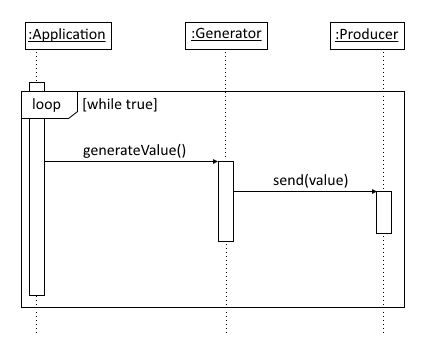
\includegraphics[width=0.75\textwidth]{bilder/sequenceProducer.png}
\caption{Sequenzdiagramm Protoyp Producer
\label{fig:seqProducer}}
\end{figure}

\begin{figure}[htb!]
\centering
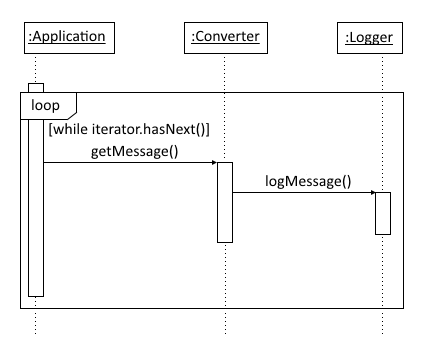
\includegraphics[width=0.75\textwidth]{bilder/sequenceConsumer.png}
\caption{Sequenzdiagramm Protoyp Consumer
\label{fig:seqConsumer}}
\end{figure}

Das folgende Kapitel beschreibt als nächstes ausgehend von den Anforderungen, den Lösungsansätzen und dem Systementwurf ein Vorgehen für die Implementierung der Prototypen und der notwendigen Zusatzanwendungen. Mit dem Anwendungsstart wird in einer Schleife dauerhaft auf Nachrichten geprüft. Sobald eine Nachricht vorhanden ist, wird die Nachricht vom \textit{Consumer} geholt und im Prototypen konvertiert. An dieser Stelle entstehen in einem Prototypen zwei Variationen. In der ersten Variation wird die empfangene Nachricht aufgenommen, es wird die Anzahl der pro Sekunde gezählt und nach jeder Sekunde wird die Anzahl der Nachricht zur nächsten Sekunde an den \textit{Logger} weitergegeben. Zu der ersten Variation kommt in der zweiten Variation zusätzlich zur Übergabe der Log-Information an den \textit{Logger} die Übergabe der Log-Information an die Übersichtsseite über \textit{WebSocket}. Dazu wird die zusätzliche Implementierung der \textit{WebSocket}-Anwendung eingesetzt. Auch der \textit{Consumer} läuft entweder im Cluster eines Streaming Framework oder in einem Systemprozess. Daher wird der \textit{Consumer}-Prozess durch den Anwender gestoppt. Nach dem der Algorithmus allgemein für den \textit{Producer} und \textit{Consumer} gezeigt wurde, wird im nächsten Kapitel das Vorgehen zur Entwicklung eines Prototypen gezeigt. Dabei wird auf Werkzeuge und Verfahren, die zur einfachen und sicheren Prototyp-Entwicklung eingesetzt werden soll eingegangen.


\section{Vorgehen}
\label{sec:vorgehen}

Bevor mit der Implementierung begonnen werden kann, ist es nötig zuerst allgemein das Vorgehen für die Entwicklung der Prototypen klar zu werden und zu beschreiben. Vor der Implementierung der Prototypen sind die Voraussetzung für ein Streaming Framework dem Grundgerüst bereitzustellen. Allgemein entspricht dem Grundgerüst eine lauffähige Fassung eines Streaming Frameworks in einem Single-Node-Cluster. Um den Prototypen bereitzustellen, zu starten und zu stoppen müssen Werkzeuge in Form von Bash-Scripts\footnote{Scripte sind Anwendungen, die in einer Shell ausgeführt werden können. Bash steht für die GNU Bourne Again SHell: \url{http://tiswww.case.edu/php/chet/bash/bashtop.html}} entwickelt werden. Da jedes Streaming Framework unterschiedliche Optionen für die Anwendung der Prototypen besitzen, werden die Bash-Scripte während dem Implementierungsprozess innerhalb eines Prototypen entwickelt.

Allgemein wird für die Entwicklung eines Prototypen zuerst mit Apache Maven eine Projekt Struktur angelegt und die Konfigurationsdatei für das Deployement eingerichtet. Anschließend wird mit Apache Maven ein Projekt für die Entwicklungsumgebung \textit{Eclipse}\footnote{Java \gls{glo:ide} Eclipse: \url{https://www.eclipse.org/}} angelegt. Da mit der Versionsverwaltung \textit{git}\footnote{Git Versionsverwaltung: \url{http://git-scm.com/}} gearbeitet wird, wird nach der Erzeugung des \textit{Eclipse}-Projekts und damit der Einrichtung des Prototypen ein initaler \textit{Commit}\footnote{Mit einem \textit{Commit} werden die Änderungen unter einem eindeutigen Referenzwert in die Versionsverwaltung aufgenommen.} in die Versionsverwaltung erstellt. Ein \textit{Commit} wird immer in einem funktionierendem Zustand des Projekts erstellt. Da \textit{git} in einem \textit{Commit} nur lokale Änderungen hinzufügt, müssen die \textit{Commits} mit dem Kommando \textit{push} an den zentralen Server übermittelt werden. In der Versionsverwaltung stehen im \textit{Repository}\footnote{Ein \textit{git} \textit{repository} bildet einen Datencontainer mit allen Änderungen, die zu einem Projekt hinzugefügt wurden.} \textit{streaming-frameworks} für die Erfassung der Änderungen zwei Zweige, der Entwicklungszweig \textit{thesis} und der Hauptzweig \textit{master} bereit. Zu Beginn jeder Woche werden die neuen Entwicklungen aus dem Entwicklungszweig in den Hauptzweig überführt und gekennzeichnet. Entwickelt wird nur auf dem Entwicklungszweig.

Die Entwicklung eines Prototypen teilt sich in zwei Teile. Der erste Teil entspricht der Implementierung einer Methode für die Prüfung von konstanten Werten. Das Logging-Framework bekommt so schnell wie möglich konstant und kontinuierlich 100-Byte große Datenpakete. Diese werden pro Sekunde gezählt und vom Logging-Framework ausgegeben. Der zweite Teil implementiert eine Methode für die Prüfung von variablen Werten. Dabei wird Text eingelesen, nach Worten getrennt, diese pro Sekunde gezählt und an das Logging-Framework weitergegeben.

Bei Fertigstellung eines Prototypen wird abschließend ein Java-Paket erzeugt und in die Versionsverwaltung hinzugefügt. Für eine binäre Datenhaltung eignet sich die Versionsverwaltung \textit{git} nicht. Unterschiede zwischen den Versionen von binären Dateien können von einer Person in einem \textit{git} \textit{repository} nicht nachvollzogen werden. Um den Aufwand klein zu halten und aufgrund der prototypischen Entwicklung, wird dennoch in \textit{git} unter dem Verzeichnis \textit{target}\footnote{In einem produktiven Betrieb muss eine andere Build- und Deployment-Strategie für die zentrale Bereitstellung von versionierten Artefakten herangezogen werden. JetBrains TeamCity \url{https://www.jetbrains.com/teamcity/} oder Jenkins \url{http://jenkins-ci.org/} ermöglichen eine kontinuierliche Integration von geändertem Quelltext.} innerhalb eines \textit{Eclipse}-Projekts die aktuelle Version hinzugefügt. 

Für das Logging wird einmalig ein Werkzeug benötigt um den Datentransport zwischen dem Prototypen und der Übersichtsseite herzustellen. Dazu wird bevor der erste Prototyp implementiert wird ein virtueller Server mit dem Apache WebServer und einer Übersichtsseite bereitgestellt. Dabei wird mit Twitter Bootstrap\footnote{Twitter Bootstrap: \url{http://getbootstrap.com/}} ein Einseitenlayout angelegt und mit Javascript werden die \gls{glo:html}-Inhalte über Javascript-Handler aktualisiert. Die Visualisierung von Diagrammen erfolgt über zusätzliche Javascript-Bibliotheken\footnote{Javascript library Data Driven Documents (D3): \url{http://d3js.org/}}. Zusätzlich wird auf der gleichen virtuellen Instanz ein NodeJs WebSocket Server bereitgestellt. Die Logging-Daten werden von den Prototypen gesendet, vom NodeJs WebSocket Server empfangen und an die Übersichtsseite per WebSocket verteilt.

Damit aus den Prototypen heraus per \textit{WebSocket} Nachrichten an den \textit{NodeJs} Server verschickt werden können, wird über eine zusätzliche Java-Bibliothek \textit{Tyrus}\footnote{Java WebSocket library Tyrus: \url{https://tyrus.java.net/}} und einem \textit{Eclipse}-Projekt ein einfaches Werkzeug implementiert. Dazu werden Java-Schnittstellen für die Konfigurationsklasse der \textit{WebSocket} Server benutzt. Die implementierten Konfigurationsklassen werden in den Prototyp-Projekt bereitgestellt und über \textit{resource}-Dateien, werden die Schnittstellen den konkreten Klassen zugeordnet. Dabei soll keine zusätzliche Bibliothek benutzt werden, sondern es wird der existierende \textit{ServiceLoader}\footnote{Java ServiceLoader: \url{http://docs.oracle.com/javase/7/docs/api/java/util/ServiceLoader.html}} für das Zusammenführen zwischen der Schnittstelle und der konkreten Implementierung aus dem \textit{Namespace} \textit{java.util} benutzt.

Das Vorgehen wurde detaillierter beschrieben und auf spezielle Aspekte, wie den zusätzlichen Werkzeugen wurde eingegangen. Im nächsten Kapitel wird eine Zusammenfassung zum Kapitel \ref{chapter:systemarchitekur} gegeben.


\section{Zusammenfassung}

Im Kapitel \ref{chapter:systemarchitekur} wurde die Entwicklung eines Prototypen beschrieben. Dazu wurden zu Beginn Anforderungen definiert und mögliche Probleme betrachtet und Lösungsansätze vorgestellt. Speziell wurde dabei auf den \gls{glo:lrb} eingegangen und in einem Teil in der Entwicklung des Algorithmus berücksichtigt. Weiterhin wurde ein Systementwurf vorgestellt. In kleinen Grafik wurde der Zusammenhang zwischen den einzelnen Komponenten aus dem Bereich \textit{Backend}, \textit{Visualization} und \textit{Display} gezeigt und erläutert. Anknüpfend darauf wurden die Geräte vorgestellt, die bei der Messung und bei der Entwicklung zum Einsatz kommen. Um die Performance des langsamsten Elements herauszufinden wurde eine Messung der Hitachi-Festplatte durchgeführt und im Anhang bereitgestellt. Zuletzt wurden aufbauend auf den Definitionen aus den Kapiteln zuvor, ein Vorgehen für das Entwickeln eines Prototypen entwickelt. Dabei wurde versucht das Vorgehen der Implementierung in den einzelnen Prototypen gleich zu halten. Im Kapitel \ref{chapter:prototypeDocumentation} werden als nächstes die einzelnen Prototypen dokumentiert.